

%\begin{sidewaysfigure}
%\centering
%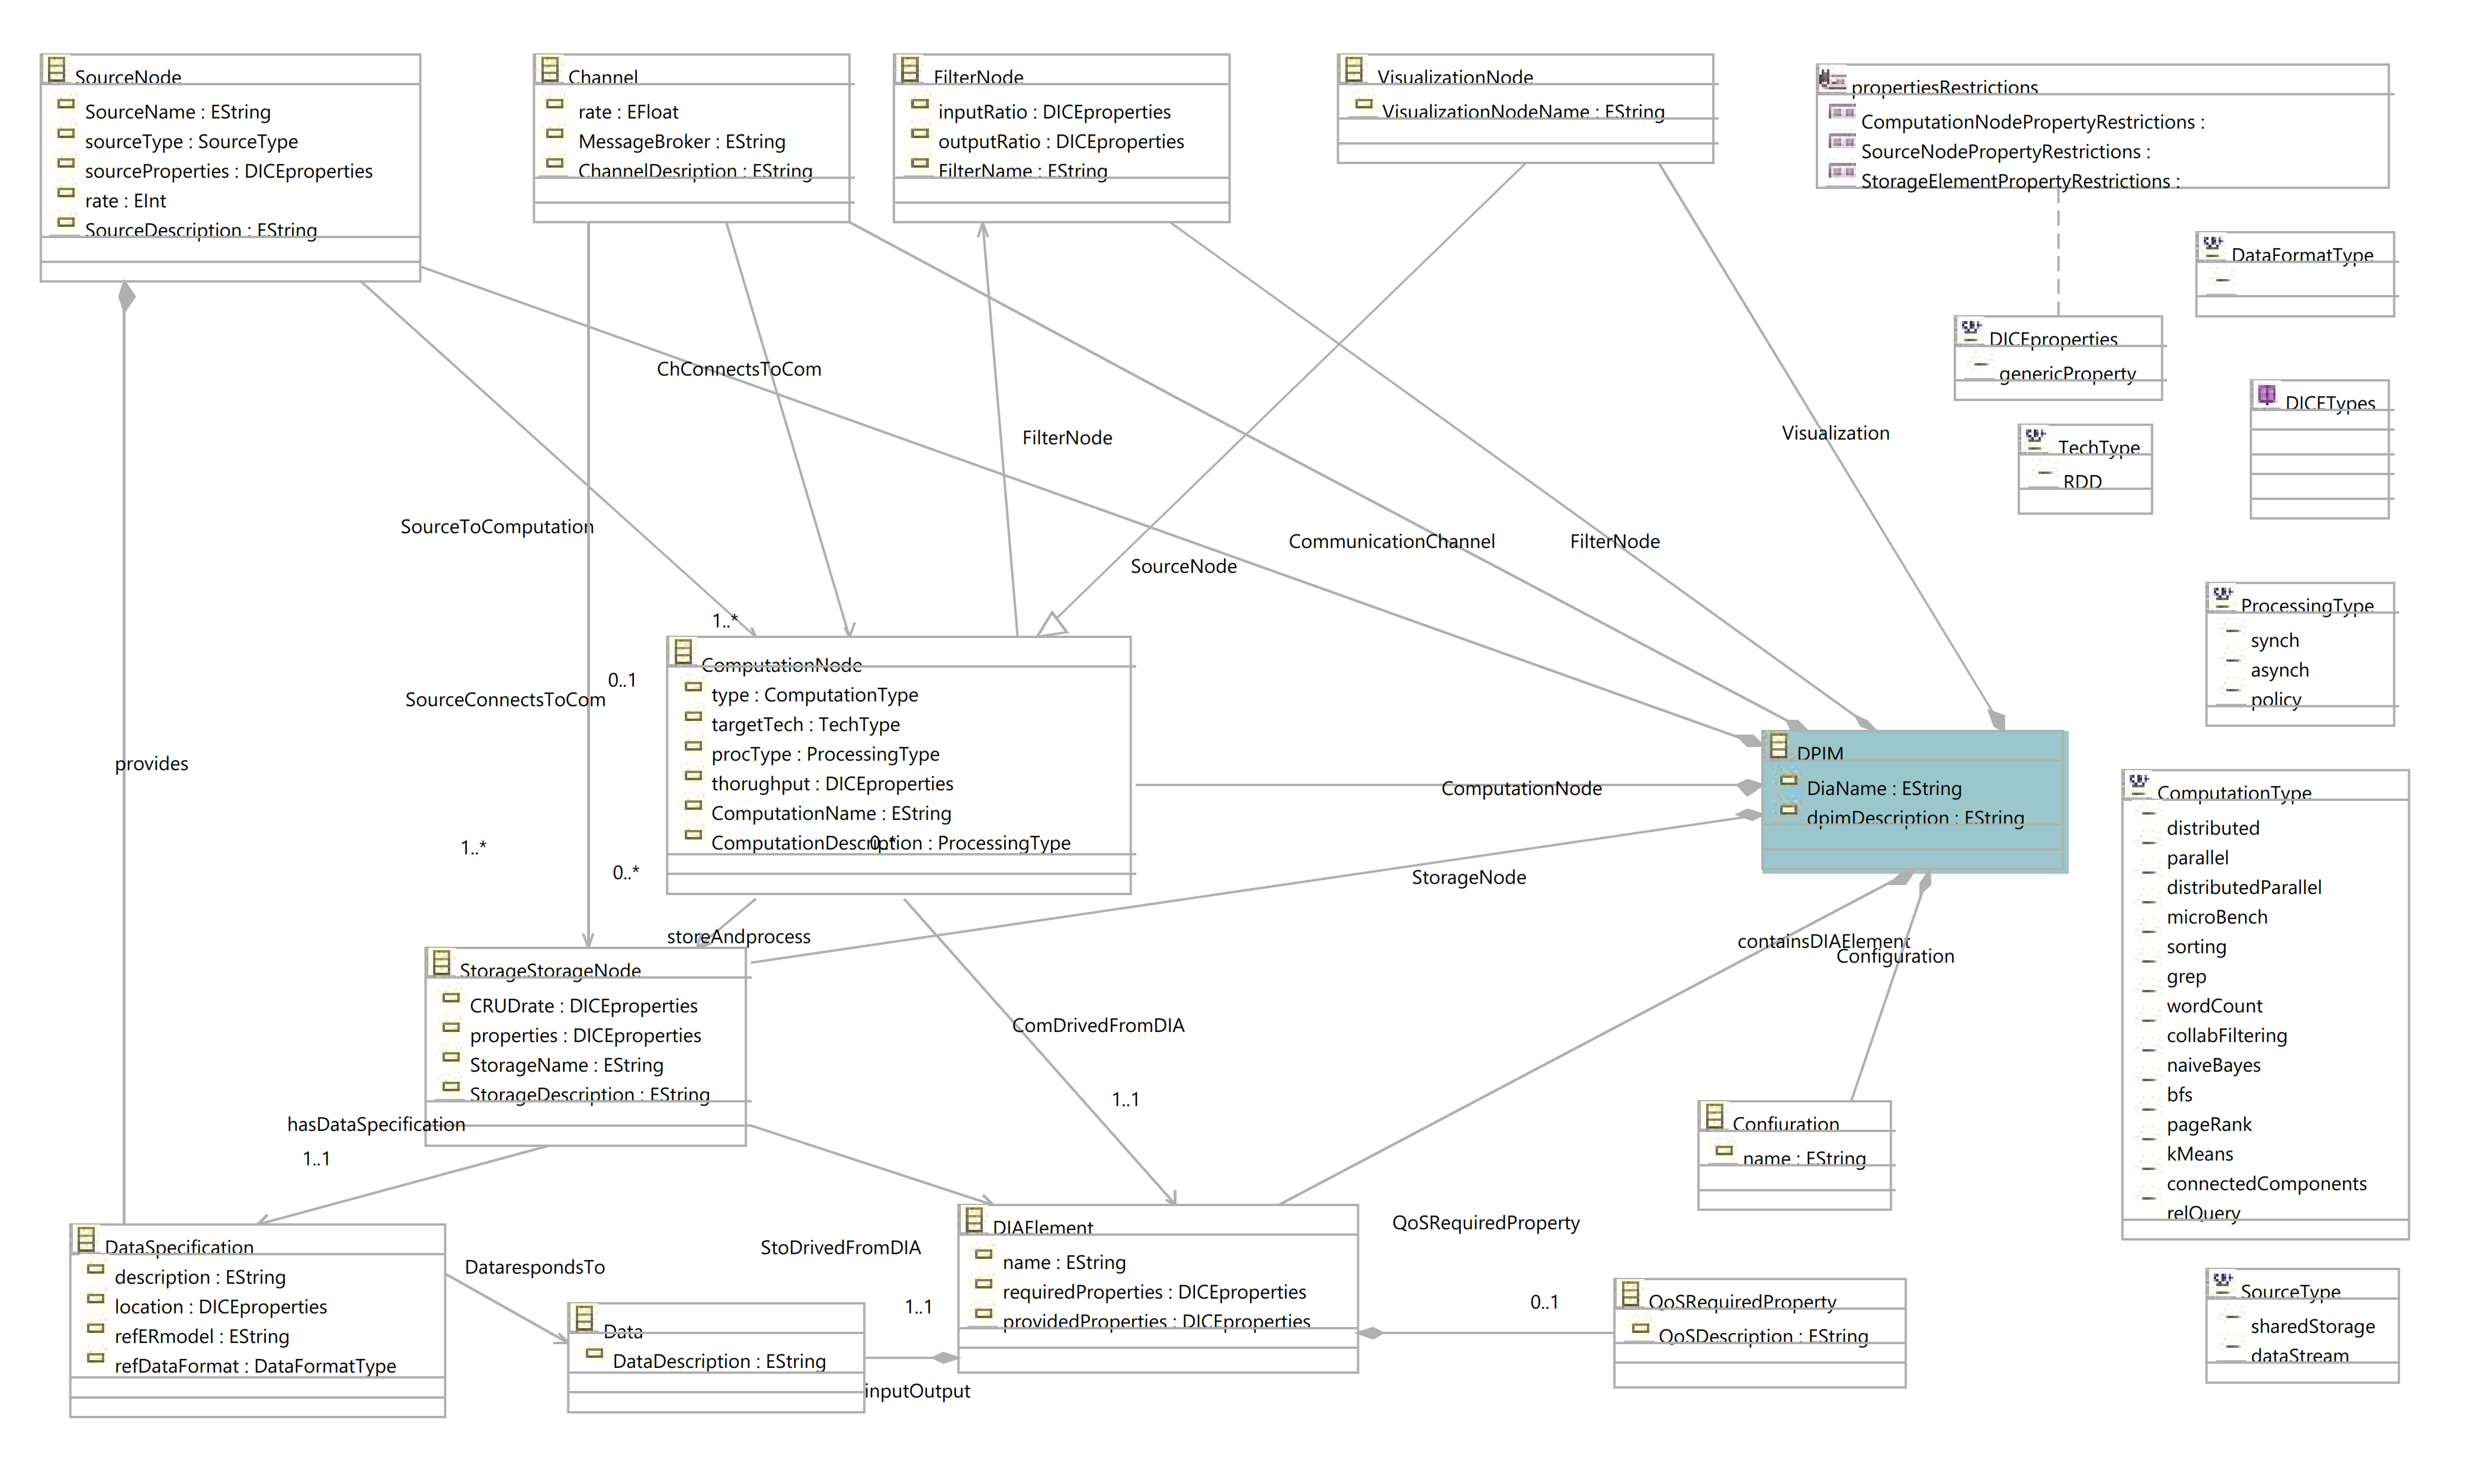
\includegraphics[width=\textwidth]{Images/11.png}
%\caption{\label{fig:metamodel}DICE DPIM metamodel.}
%\end{sidewaysfigure}

%\begin{figure}
%\centering
%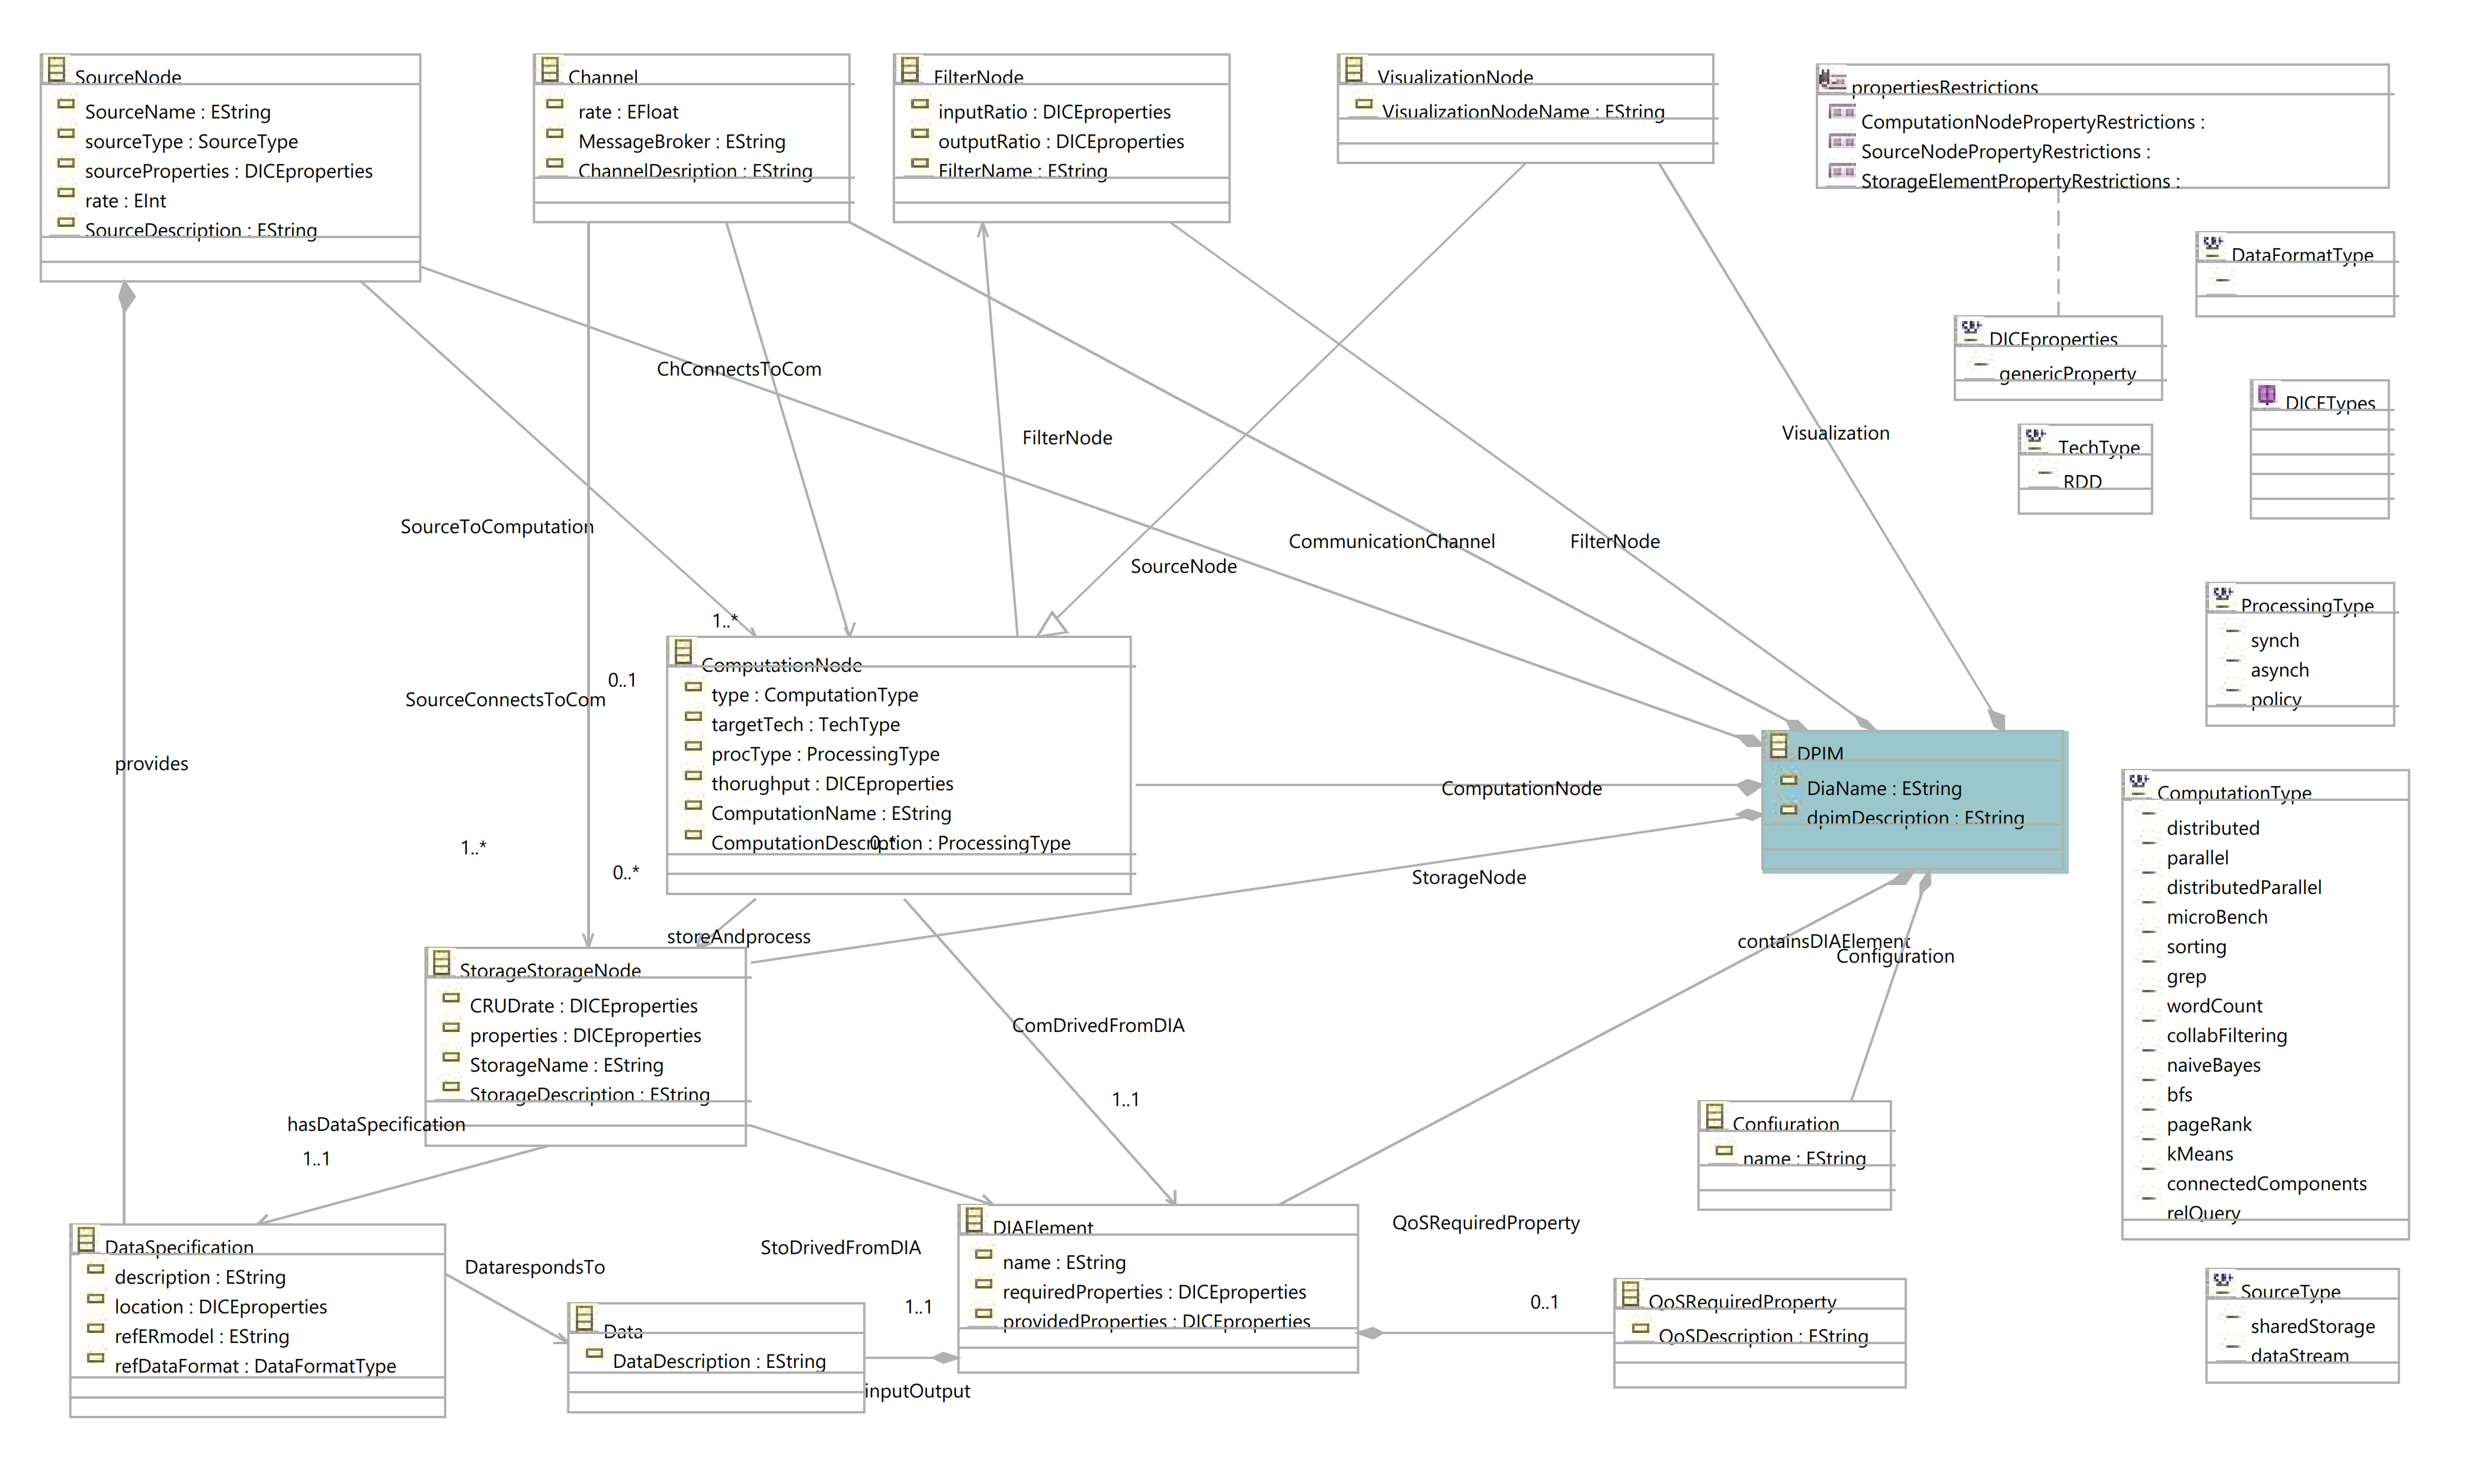
\includegraphics[width=\textwidth]{Images/11.png}
%\caption{\label{fig:metamodel2}DICE DPIM metamodel in portrait form.}
%\end{figure}

\subsection{Product perspective }

\subsubsection{Class Diagram}
The following class diagram is a high-level class diaram which should be intended as a model of the application structure. During the implementation part more classes and attributes can be created and used.

%Sideway figure
%\begin{sidewaysfigure}
%\centering
%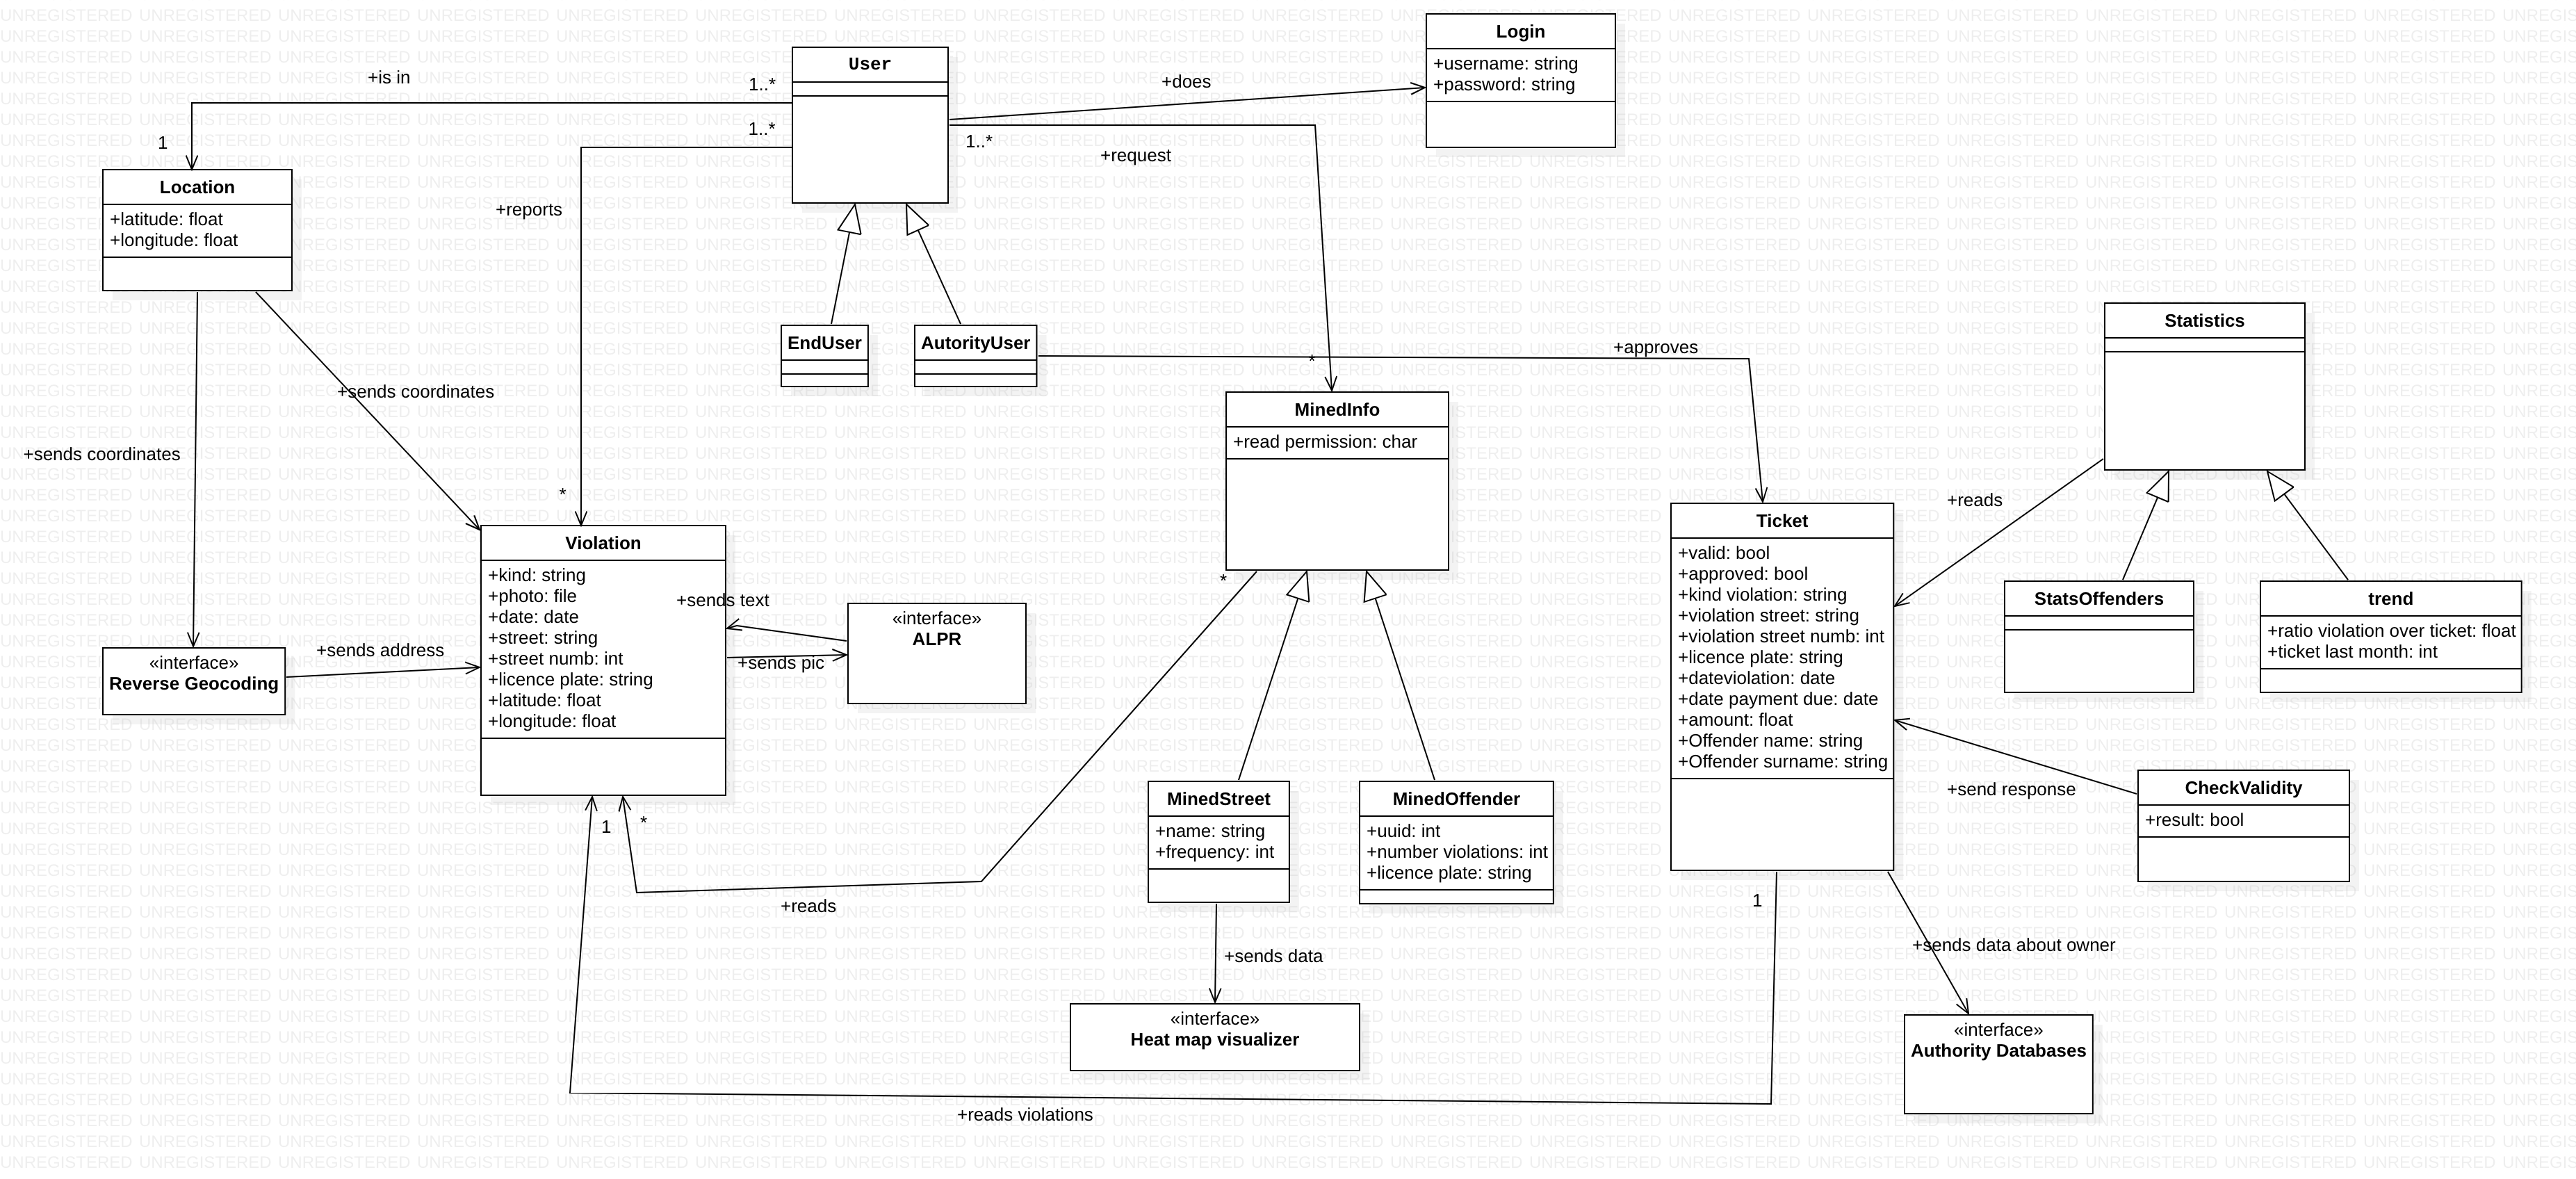
\includegraphics[width=\textwidth]{Images/Class.png}
%\caption{\label{fig:classdiagram}High-level Class Diagram}
%\end{sidewaysfigure}

\begin{figure}
\centering
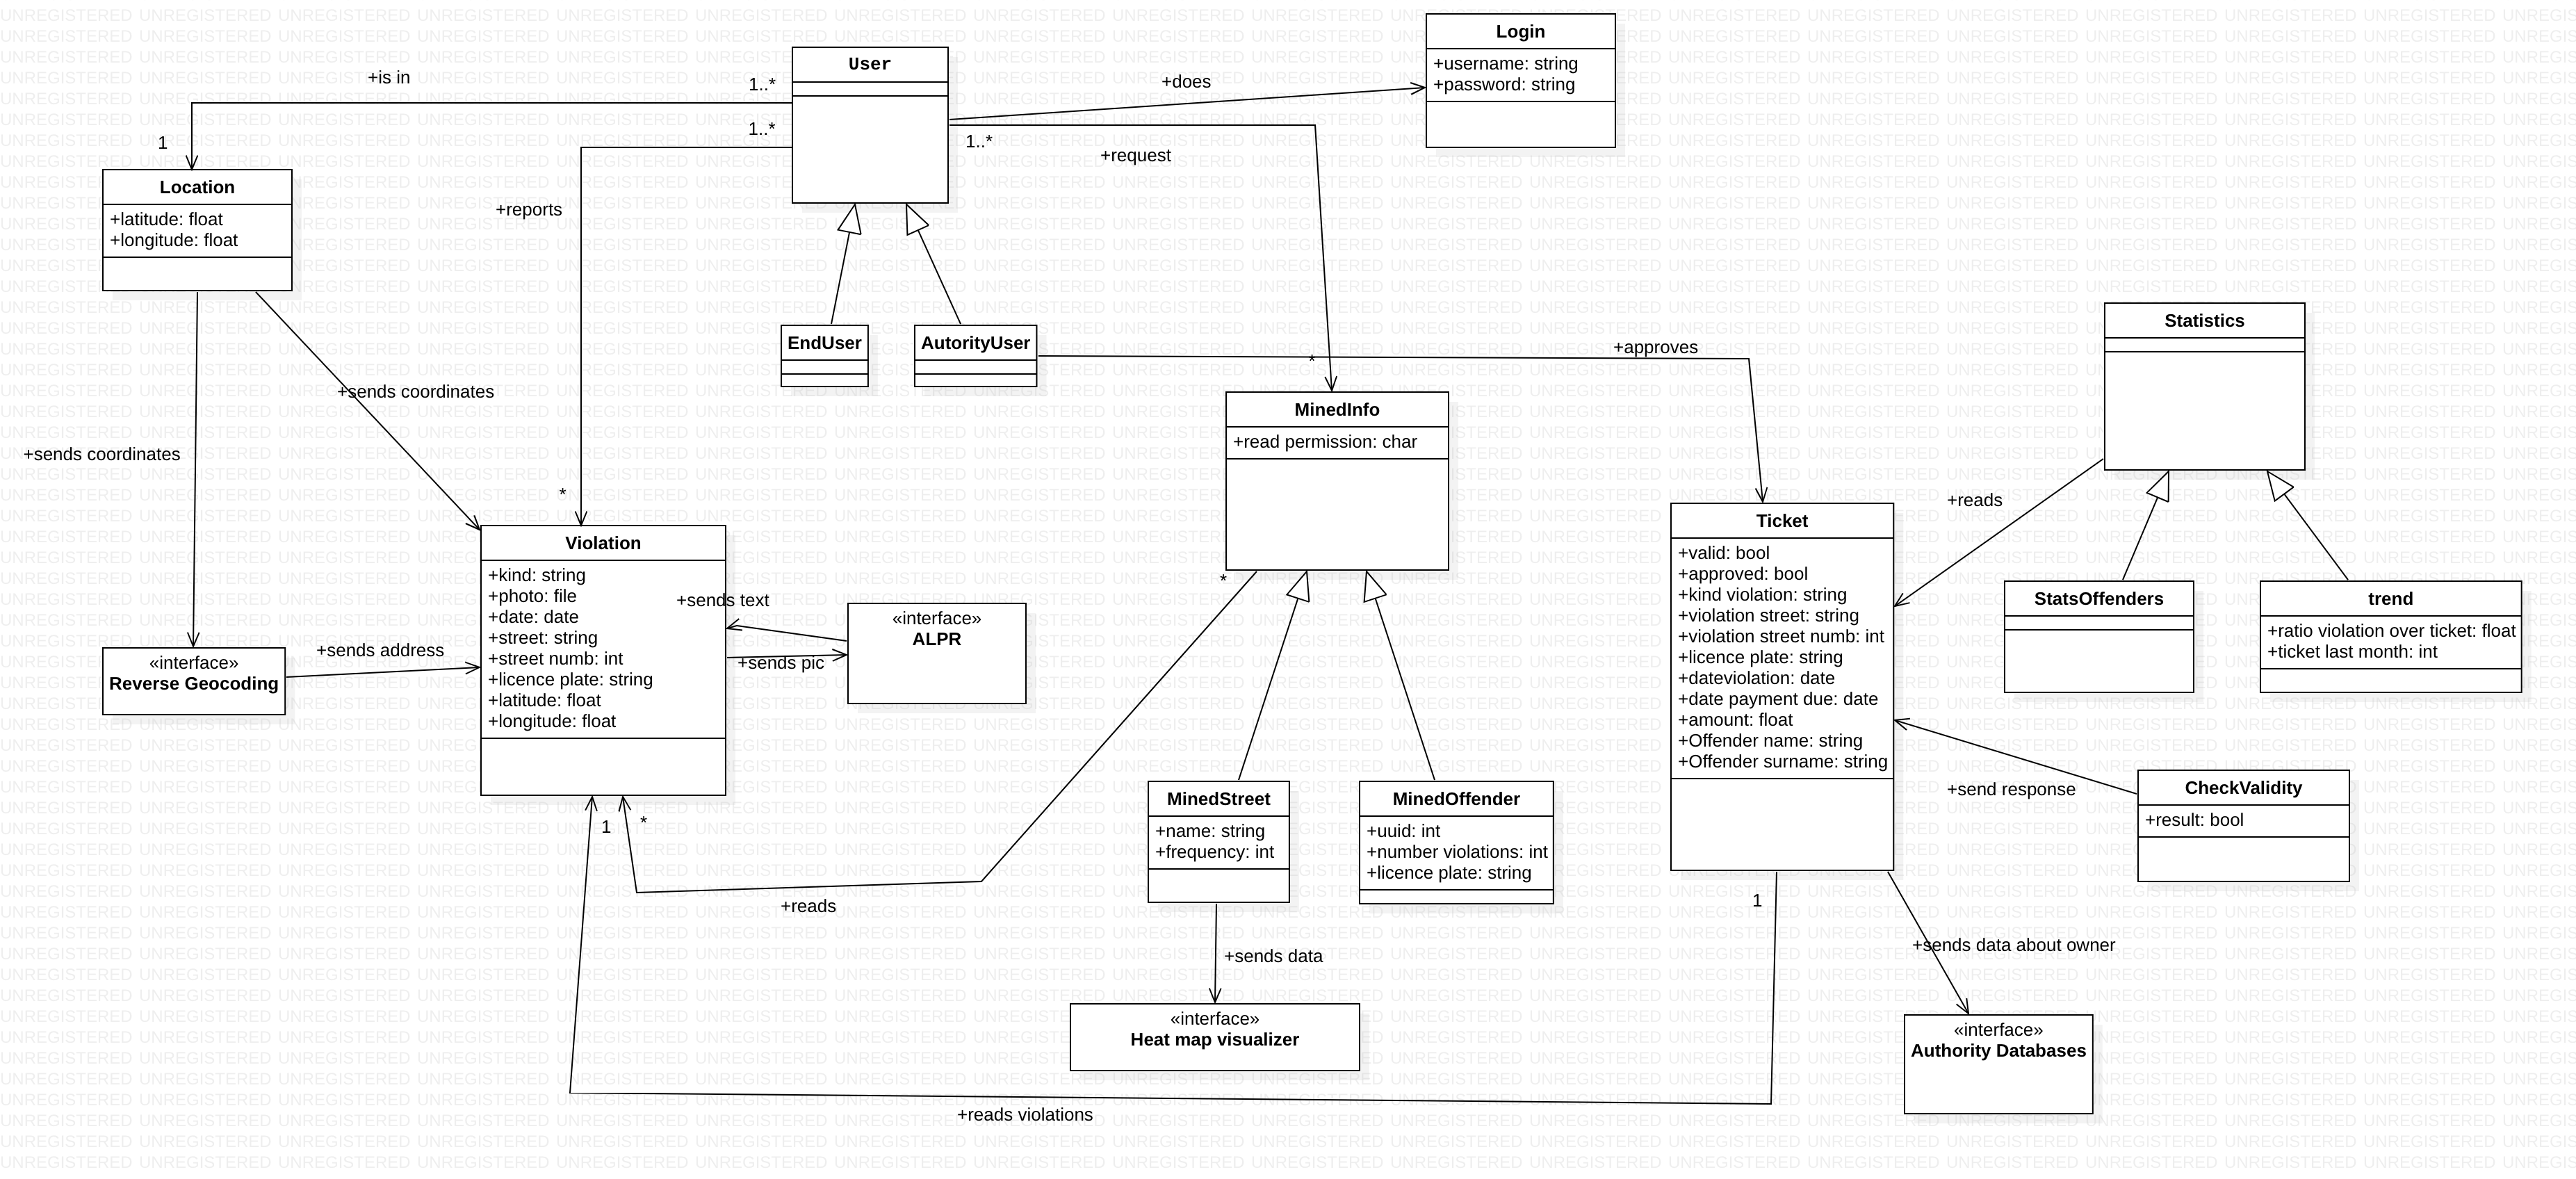
\includegraphics[width=\textwidth]{Images/Class.png}
\caption{\label{fig:classdiagram}High-level Class Diagram}
\end{figure}



\paragraph{User}
This class is the father of the two possible kind of users: \textbf{EndUser} and \textbf{Authority} which are needed because our application is intended to be multi-user and with at least two priviledges for data that can be viewed and possible functions accessible.
\paragraph{Location}
Every user is in a \textbf{Location} class used to represent the location as latitude and longitude coming from the SO of the smartphone.
\paragraph{Reverse Geocoding}
This interface is used to communicate with the external serveice to get a readable address from the coordinates as explained in section \ref{Dependencies}.
\paragraph{Violation}
This class is used to store all the data relative of the reported violation. The \textit{kind} attribute is selected by the user in the fill form from a list of possible kind of violations, see use case \ucas{}.
The photo is here reported an attribute but can also be implemented as a separate class. It's mandatory that one picture is associated to every violation. In the \textbf{Violation} class there are also stored the raw latitude and longitude in case there will be need of those data later, as an example if it's imposssible get precise location using reverse geocoding.
\paragraph{ALPR}
This interface is needed to interact with the external ALPR service which receives a picture and returns a string containing every licence plate found in the picture. This interface is used to complete the attribute \textit{licence plate} of every violation.
\paragraph{MinedInfo}
Classes \textbf{MinedSteets} and \textbf{MinedOffenders} are used to represent the data coming from the database of all violation and processed to offer different kind of visualization.
\paragraph{Heat Map visualizer}
This interface is used to communicate with the external service providing a map of streets with an overlay highliting the spots where violation occurred.
\paragraph{Ticket}
this class is used to represent the ticket with the fine for the owners of violationg veichles. every instance will be automatically creadted by the system, using data coming from the instances of the \textbf{Violation} class.






%add a state diagram for each subsect


\subsection{Product functions}

\subsubsection{Report violation}

\subsubsection{Explore Data}
The app will offer the possibility to the users to visualize the data collected.
Two kind of visualizations are offered:
\begin{enumerate}
  \item Heatmap of streets where most violations occurred
  \item Vehicles that committed the most violations
\end{enumerate}
In order to get those data the system will periodically query the database of violations in order to create a table where the count of violation is stored, both for streets and vehicles.
There will be a section in the app called "Explore Data" where will be able to choose which kind of data to visualize.

\subsubsection{subsubsection name}


\subsubsection{Issue a ticket}
\begin{figure}
\centering
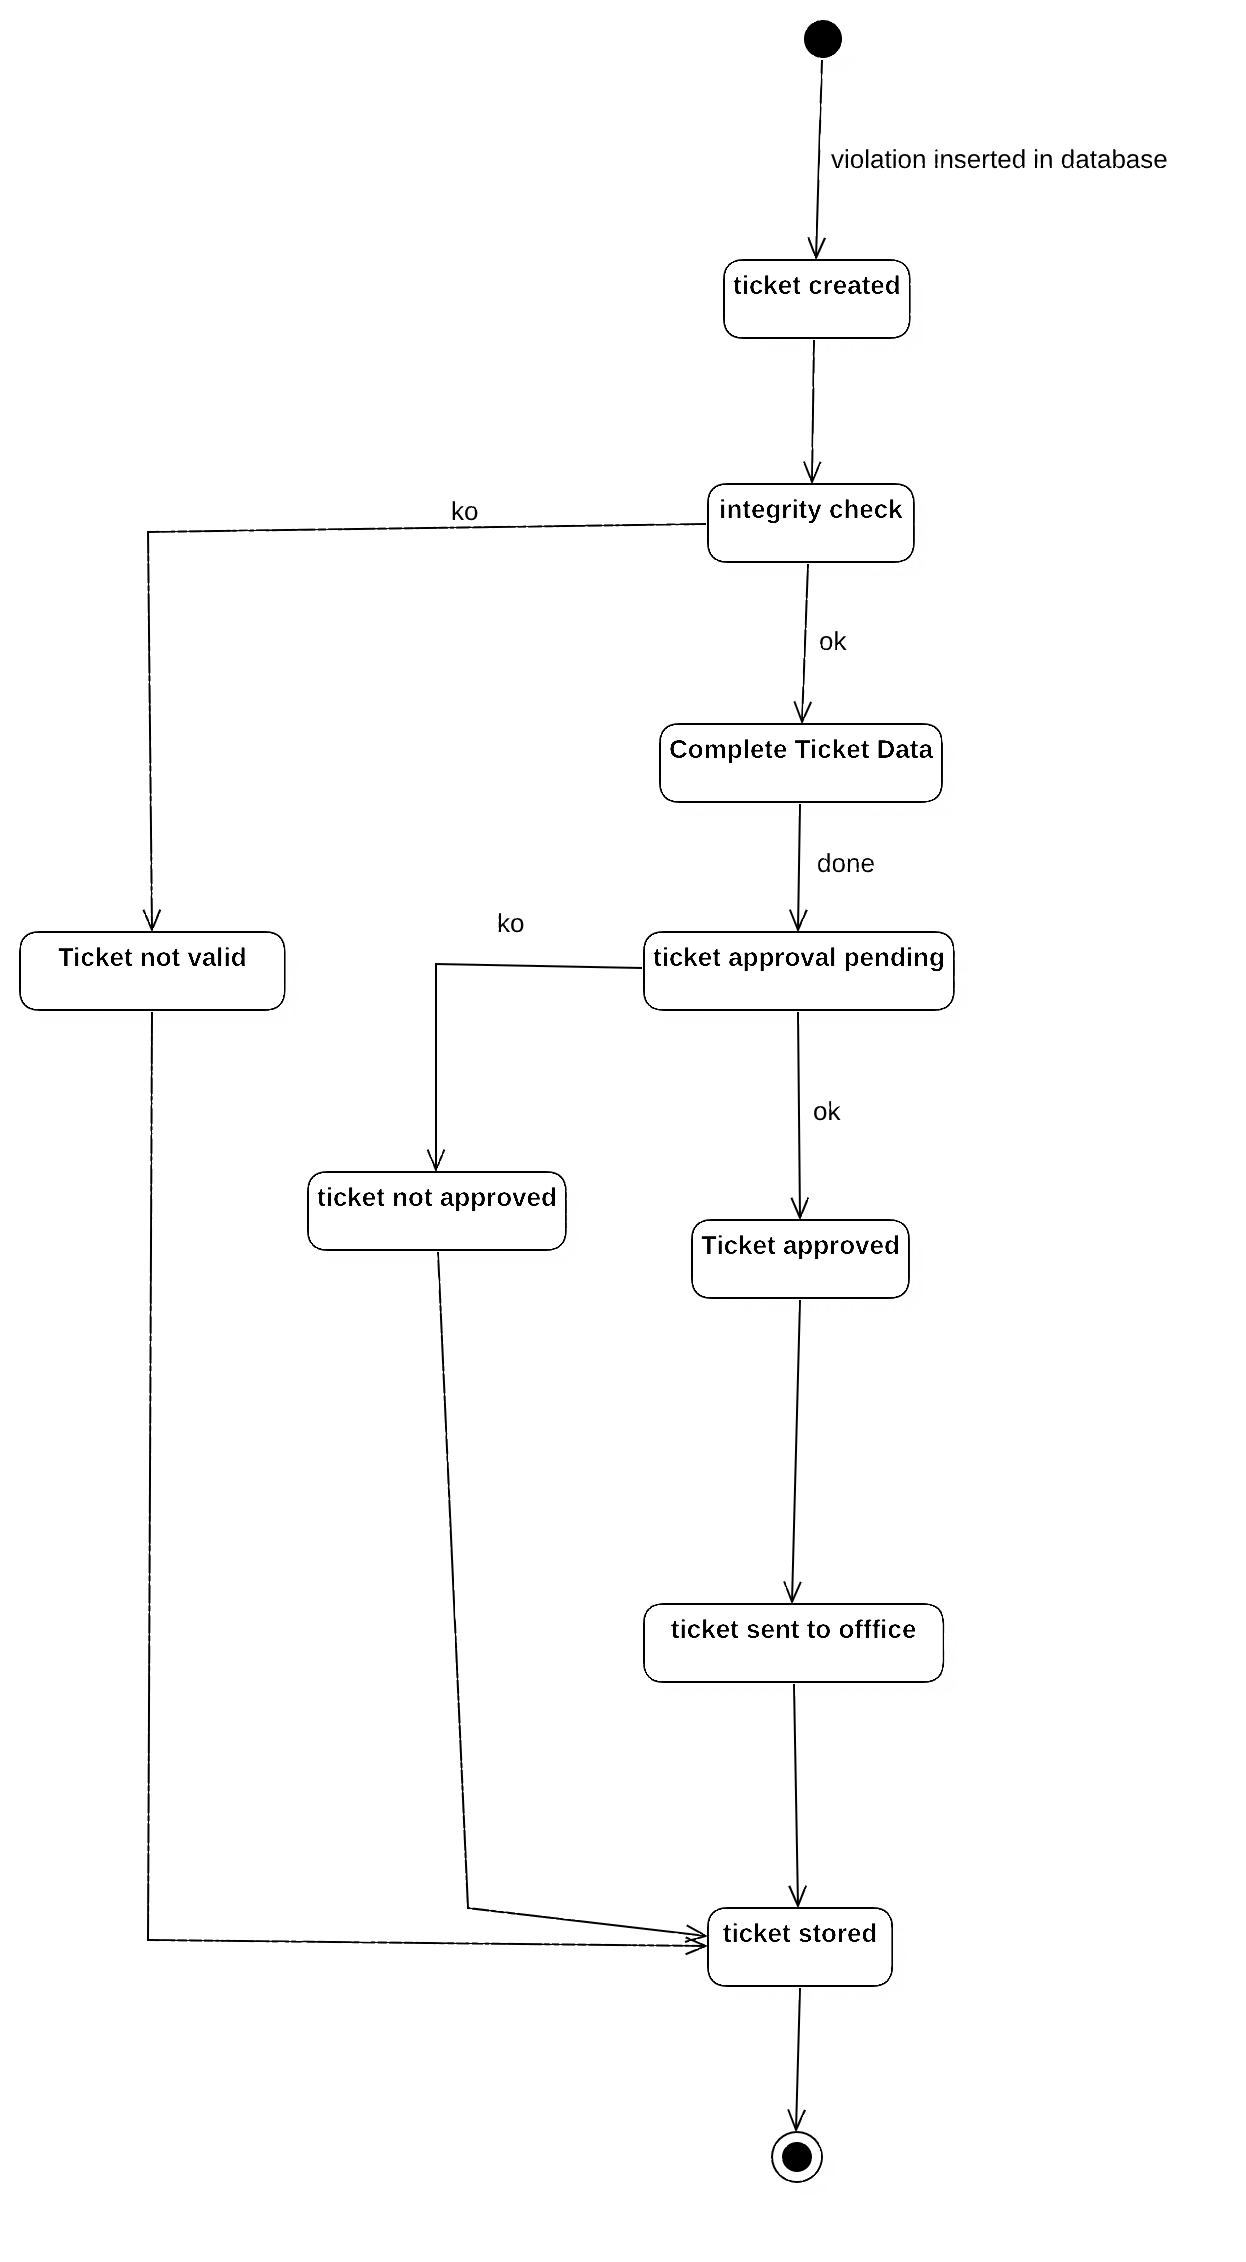
\includegraphics[width=0.7\textwidth]{Images/ticketstate.png}
\caption{\label{fig:ticketstatediag} Tickets creation and approval state diagram}
\end{figure}

This function is used to create tikets to send fines to the owners of veichles which have been reported by SfeStreets.
Every time a new violation is inserted in the database the System will use the new data available to generate a proposal of ticket, combining the data from violations with data coming from Municipality databases.

A ticket has the following structure:
\begin{enumerate}
  \item Place where violation occurred
  \item Date when violation occurred
  \item Plate of veichle
  \item Article and code of violation
  \item Amount to be paid
  \item Date when the payment is due
\end{enumerate}

Place, date, plate are data coming from the instances of Violation class. To create a complete ticket we need to associate the kind of violation to an article and code of the traffic legislation.

An external service or a code writted ad hoc will be used to check if the picture has been modified.
If the result of this check is positive the ticket just created will be flagged as \textit{valid} and will go in ticket approval state.
In any other case, if the picture has been modified, the ticket is stored as \textit{not valid} for debug purposes. Exaples of possible uses can be: bulding statistics or investigate if there are users who are trying to cheat or create spam violations.

If a ticket is considered valid, the next state is pending-approval status.
Authority users (e.g. policemen) will check manually the pending-approval tickets reading all data before the approval. We have chosen to add this human control before sending the fine because every ticket should be signed by authorities. If ticket is not approved it will go in approval-denied status and will be stored for debug purposes and for statistics.

If ticket has been approved it will have to be sent to the offender.
The system will connect to the external vehicle registration database in order to retrieve the name, surname, address of the offender knowing the licence plate of his/her vehicle.
Now we have all the data to print the ticket and send it via regular mail. There will be an office of police-station which will do the job.

\subsubsection{Generate statistics}

\subsection{User characteristics }

\subsection{Assumptions, dependencies and constraints}
\subsubsection{Domain assumptions}

\begin{enumerate}
\dom{1}  Device has internet connection
\dom{1} The device should acquire position with an accuracy of enouth meters in order to univocally determine the road (e.g. 5 meters)
\dom{} We have access to an ALPR service which is able to read every licence plate in a picture and return the string
\dom{1} The device should take pictures with enough resolution to be able to read by the ALPR service
\dom{5} ALPR service has an accuracy of more than 90\%
\dom{2} Every vehicle that can be reported should have a licence plate visible
\dom{3} The number and kind of violations should be finite (defined by the law)
\dom{4} Every authority account is verified and it's not possible to be created using the front end
\dom{6} We have access to the vehicle registration database where are stored licence plates, names and the addresses of the owners of every vehicle registered
\dom{7} We have access to a database where are stored all the codes of violations and the amount of fine for the violation

\end{enumerate}

\subsubsection{Dependencies} \label{Dependencies}

The app will be dependent on a third-party service to read the licence plate of the cars

the app will be dependent on some Maps API to get the full address, knowing the coordinates of location coming fromm the GPS of the device.

The app will be dependent to some Maps API used to show the map and an overlay.



The app will be dependent on a smartphone, which has to provide the following features:
\begin{enumerate}
  \item Internet connection, possibly using 2G/3G/4G in order to be available where there is no WiFi, considering the use case "on the road"
  \item A camera with good resolution
  \item GPS sensor
\end{enumerate}
